\Chapter{Modélisation par les vitesses de dérive}
\chaptermark{Les vitesses de dérive}
\begin{refsection}
Le deuxième chapitre de cette thèse concerne la modélisation du transport
(fortement) magnétisé par une approche basée sur les vitesses de dérive. Cette
méthode, élaborée dans le cadre de la recherche sur la fusion par
confinement magnétique, est implémentée dans TOKAM2D~\cite{Sarazin}, un code 
spécifiquement développé pour caractériser le transport dans le plasma de bord
des tokamaks.

Nous introduisons tout d'abord le code TOKAM2D et les hypothèses sur
lesquelles repose le modèle. Les équations de continuité et de
courant sont ensuites dérivées avec quelques précisions sur les approximations
choisies.
Dans une deuxième partie, nous présentons les évolutions du
modèle et les modifications entreprises sur le code pour lui
permettre décrire le transport dans des conditions caractéristiques aux plasmas
froids. Sont ainsi passées en revues :

\begin{itemize}
  \item l'inclusion de conditions aux limites
perpendiculaires
\item la prise en compte de géométries de champ magnétique complexes
\item l'ajout de l'équation de la
température électronique
\item la construction d'un modèle basé sur les vitesses de dérive pour les plasmas froids
\end{itemize}

Pour le dernier point, les équations sont redérivées en tenant
compte du transport collisionnel avec les neutres. Le modèle intègre de plus des
conditions aux limites de type gaine sur le courant et le flux de particules
dans la direction perpendiculaire au champ magnétique.

\section{Le code TOKAM2D}

\sectionmark{Le code TOKAM2D}
La première année de cette thèse a consisté à utiliser et modifier le
code {TOKAM2D}. Le but était alors de se familiariser avec les
techniques développées pour la modélisation des plasmas
de SOL et les mécanismes du transport magnétisé afin
de pouvoir les appliquer au problème des sources d'ions. 

Le code TOKAM2D est un code fluide, quasineutre, qui décrit le transport
transverse en se basant sur l'approximation des vitesses de dérive (voir §
\ref{Introduction}-\ref{vitessesDerive}). Initialement développé à
l'Institut Méditerranéen Technologique de Marseille (IMTM) pour étudier
la turbulence d'interchange, sa modification pour intégrer un forçage de la turbulence
par un flux au lieu d'un gradient d'équilibre a permis de retrouver le
caractère intermittent du transport et la longueur de décroissance du profil de
densité que l'on mesurait expérimentalement~\cite{SarazinPhD}. L'étude du modèle a
ainsi permis d'améliorer la compréhension du mécanisme de l'instabilité
d'interchange, par la mise en évidence du transport turbulent de type
avalanche. Il a aussi aidé à prouver le déclenchement à seuil de
l'instabilité.

\subsection{Hypothèses du modèle}
Dans les conditions typiques de la SOL, l'utilisation d'un modèle fluide est
justifiée par la forte collisionnalité du plasma. Le libre parcours moyen
$\lambda_{ei}=v_T \nu_{ei}$, de l'ordre du mètre, est très inférieur à la
longueur de connexion parallèle des lignes de champ $L_\para\sim
$~100m.

Le plasma est de plus très magnétisé $B\sim$~1T, les fréquences
caractéristiques du transport transverse sont donc suffisement lentes devant la
fréquence cyclotronique ionique pour nous placer dans le cadre de
l'approche par vitesses de dérive :

\begin{equation}
\omega\ll\omega_c\Leftrightarrow \varepsilon_\omega\equiv\frac{\omega}{\omega_c}\ll 1
\end{equation}

D'un autre côté $\rho\indice{i}$, le rayon de Larmor ionique, d'environ
1mm, est bien supérieur à la longueur de
Debye $\lambda_D$, de l'ordre de 10$^{-5}$~m, ce qui autorise à
considérer le plasma quasineutre dans son ensemble, avec des densités ionique
et électronique équales à $n$.
Le transport est alors décrit à travers l'évolution de la densité
électronique $n$ et du potentiel électrostatique $U$ en résolvant l'équation
de continuité des électrons ainsi que l'équation de conservation du courant. Les
températures électronique
$T_e$ et ionique $T_i$ sont supposées constantes, avec un rapport $\tau=T_i/T_e$.

\begin{figure}[htbp]
\centering
    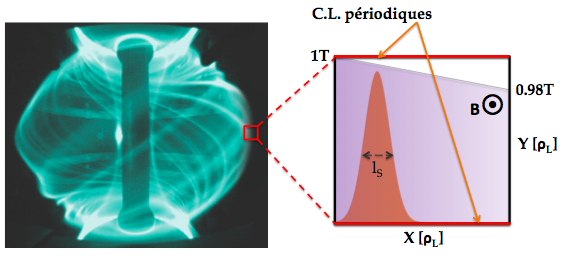
\includegraphics[width=0.8\textwidth]{figures/2-tokamSimDomain.png}
    \caption{La région simulée est située à la frontière du plasma confiné,
    au niveau de la séparatrice, et dans le plan poloïdal médian.}
    \label{2-figTokamGeom}
\end{figure}

L'hypothèse flûte, qui sera développée §\ref{2-flute}, permet enfin de réduire
le problème de trois à deux dimensions.
La figure~\ref{2-figTokamGeom} montre la zone simulée. La SOL est représentée
en géométrie slab, ie. avec $x\equiv(r-a)/\rho_\text{L}$ et $y\equiv
a\theta/\rho_\text{L}$ les coordonnées transverses, normalisées par le rayon
de Larmor ionique. La séparatrice est modélisée par un flux entrant de particules,
qui sépare la zone simulée en deux régions :

\begin{itemize}
  \item une région stable, ie. où la courbure magnétique est favorable, à gauche
  de la source
  \item une région sujette à l'instabilité d'interchange (côté LFS) à droite
 \end{itemize}
 
Dans la version initiale de TOKAM2D, pour des raisons pratiques, le domaine de
simulation a été choisi bipériodique. 

\subsection{Dérivation des équations}
\subsubsection{Equation de conservation de la matière}
La densité $n$ du plasma est conrôlée par l'équation de continuité des
électrons. L'effet des collisions coulombiennes est pris en compte à travers un
terme diffusif de coefficient $D_\perp\sim eT_\text{e}/m_\text{e}\nu_\text{ei}$
et on note $S$ un terme source modélisant le flux de particules
provenant du plasma de c\oe{}ur. L'équation de continuité s'écrit :

\begin{equation}
\label{2-ContinuiteElectrons}
\partial_t n + \nabla\cdot(n\mathbf{u}) = D_\perp\nabla^2_\perp n + S
\end{equation}

En décomposant la divergence suivant les directions parallèle et
perpendiculaire, et en se souvenant que le flux de matière transverse est
essentiellement issu de l'advection par la vitesse de dérive électrique
(cf.~§\ref{Introduction}-\ref{vitessesDerive}), \eqref{2-ContinuiteElectrons} peut se développer en :

\begin{equation}
\label{2-ContinuiteElectrons2}
\partial_t n + \nabla_\para(nu_{\para}) =
\mathbf{u}_E\cdot\nabla_\perp n + D_\perp\nabla^2_\perp n + S
\end{equation}

Le terme d'advection $\mathbf{u}_E\cdot\nabla_\perp
n$ se réécrit en utilisant la notation
du crochet de Poisson $[n,U]=\mathbf{b}.(\nabla_\perp n\times\nabla_\perp U)$.
C'est la forme que prend toute advection d'un champ scalaire par une vitesse de
dérive $\mathbf{v}_\text{D}=\nabla H\times\mathbf{B}/B^2$, où $\nabla H$ est la
force à l'origine de la dérive. L'équation de continuité pour les électrons
s'écrit alors :

\begin{equation}
\label{2-eqContinuiteFinale}
\partial_t n + \nabla_{\para}(nu_{\para}) =
\frac{1}{B}\left[n,U\right] + D_\perp\nabla^2_\perp n + S
\end{equation}

Le terme non-linéraire $[n,U]$ est l'un des éléments moteur du modèle
d'interchange. Couplant la densité au potentiel électrique, il opère un
transfert d'exitation des composantes radiales des fluctuations à leurs
composantes poloïdales et réciproquement. Les termes de flux parallèle et de
diffusion sont stabilisant, ils tendent à
amortir les fluctuations et donc à homogénéiser le système.

\subsubsection{Equation de conservation du courant}
L'équation de conservation du courant s'obtient en soustrayant l'équation de
continuité des électrons à celle des ions. La vitesse de dérive électrique
$\mathbf{u}_E$, indépendante de la masse et de la charge des particules,
est identique pour les deux espèces et ne transporte donc aucun courant. 
La conservation du courant se résume ainsi à un équilibre entre le courant
parallèle $\mathbf{j}_\para$ et les courants transverses diamagnétique
$\mathbf{j}_*$ et de polarisation $\mathbf{j}_p$ à travers leur
divergences:

\begin{equation}
\label{EqCourant1}
\nabla\cdot\left(\mathbf{j}\right) = 
\nabla\cdot\left(\mathbf{j}_\para+\mathbf{j}_*+\mathbf{j}_p\right)
= 0
\end{equation}

La divergence du courant diamagnétique, dans un plasma isotherme, donne un
crochet de Poisson entre la densité et la courbure du champ magnétique :

\begin{equation}
\nabla\cdot\mathbf{j}_*=
\nabla_\perp\cdot\left(\nabla_\perp\left(
P_i+P_e\right)\times\mathbf{B}/B^2\right) =
T_e(1+\tau)\left[n,B\puissance{-1}\right]
\end{equation}

La vitesse de polarisation étant de plus
proportionnelle à la masse des particules \eqrefp{1-vitessePol}, on ne
retient dans l'expression du courant que la contribution ionique :
\begin{equation}
\mathbf{j}_p\sim\text{e}n\mathbf{u}^i_p=-\frac{nm_\text{i}}{B^2}\frac{\text{d}\nabla_\perp
U}{\text{dt}}
\end{equation}

En exprimant la dérivée totale de
façon eulérienne, la divergence du courant de polarisation devient :
\begin{equation}
\nabla\cdot\mathbf{j}_p\sim\nabla\cdot\left(\text{e}n\mathbf{u}^i_p\right)\equiv
-\nabla_\perp\cdot\left(\frac{nm_\text{i}}{B^2}\left(\partial_\text{t} -
\nu_\perp \nabla_\perp^2 +
\mathbf{u}\cdot\nabla_\perp\right)\nabla_\perp U\right)
\end{equation}
$\nu_\perp$ représentant une viscosité effective du milieu\footnote{L'origine
physique de cette viscosité définie par le coefficient $nu_\perp$ peut être
rapprochée de la conductivité de Spitzer $\eta\equiv
n_\text{e}e\puissance{2}/m_\text{e}\nu_\text{ei}$, soit encore à une expression
modifiée de la vitesse de dérive électrique
$\mathbf{u}_\text{E}=(1+\rho_\text{L}\puissance{2}/4\nabla\puissance{2})\mathbf{E}\times\mathbf{B}/B\puissance{2}$}.
De manière similaire à \eqref{2-ContinuiteElectrons2}, seule l'advection par la
vitesse de dérive électrique est considérée dans la divergence : 
$\nabla\cdot\left(\mathbf{u}\,\nabla_\perp^2 U\right)
\approx\nabla\cdot\left(\mathbf{u}_E\,\nabla_\perp^2 U\right)$.
En insérant l'expression des dérives, \eqref{EqCourant1} se réécrit :

\begin{equation}\begin{split}
\label{EqCourant2}
\nabla_\para j_\para +
T_e(1+\tau)\left[n,B\puissance{-1}\right] + \nabla_\perp\cdot\left(-\frac{nm_\text{i}}{B^2}\left(\partial_\text{t}\nabla_\perp
U - \nu_\perp \nabla_\perp^3 U \right)\right) \\+
\nabla_\perp\cdot\left(-\frac{nm_\text{i}}{B^2}\mathbf{u}_E\cdot\nabla_\perp^2
U\right)=0
\end{split}
\end{equation}

Diverses considérations sur l'importance relative des termes contenus dans
\eqref{EqCourant2} (reliées aux hypothèses d'ordering
et aux variations de champ magnétique) sont développées dans
\cite{SarazinPhD}. En effectuant un changement de variable $W=\nabla_\perp^2U$, où $W$ symbolise
une vorticité\footnote{La vorticité d'un écoulement est généralement définie comme le rotationnel de sa vitesse. Dans la SOL, le champ de vitesse correspond essentiellement à la dérive ExB, ce qui donne pour un
champ magnétique constant de 1T : 
$\nabla\times\mathbf{v}\sim\nabla\times\mathbf{u}_E=\nabla\times(\mathbf{E}/B\times\mathbf{b})\equiv-\nabla_\perp^2
U=W$ }, \eqref{EqCourant2} se transforme en :
\begin{equation}\begin{split}
\label{2-eqCourantFinale}
\nabla_\para{j}_\para +
T_e(1+\tau)\left[n,B\puissance{-1}\right] =\\
\frac{nm_i}{B^2}\left(\partial_\text{t}W - \nu_\perp
\nabla_\perp^2W+
B\puissance{-1}\left[U,W\right]\right)
\end{split}
\end{equation}
une équation simplifiée dite de vorticité. 

 Dans le système d'équations
 \eqref{2-eqContinuiteFinale}~--~\eqref{2-eqCourantFinale}, seules restent
 inconnues la vitesse parallèle électronique  et le courant parallèle. La
 fermeture s'opère alors en moyennant les équations le long de la direction
 parallèle. 

\subsection{Système moyenné et normalisation}
\label{2-flute}
\subsubsection{Réduction 2D}

 L'hypothèse flûte, qui s'appuie sur des observations
expérimentales\footnote{Des mesures expérimentales ont montré que le vecteur
d'onde parallèle des fluctuations électrostatiques était très petit devant la
longueur de connexion parallèle $L_\para$\parencite{Woot90}}, consiste à
considérer les fluctuations constantes le long des lignes de champ. Toute grandeur $f(x,y)$
vérifiant l'hypothèse flûte est donc indépendante de la direction parallèle et
sa moyenne est égale à la fonction elle-même :
\begin{equation}
\left<f(x,y)\right>_\para=f(x,y)
\end{equation}
En supposant que la densité $n$ et le potentiel $U$ ne dépendent que de x et de
y, le passage des équations
\eqref{2-eqContinuiteFinale}~--~\eqref{2-eqCourantFinale} à la moyenne laisse
la plupart des termes inchangés.

Les divergences parallèles du flux et du
courant font naturellement apparaître
les conditions aux limites de gaine issue du critère de Bohm (cf.~\ref{1-gaine})
:
\begin{align}
\left<\nabla_\para
nu_\para\right>_\para&=\frac{nc_s}{L_\para}\exp(\Lambda-\Delta\Phi/T_e)
\\
\left<\nabla_\para
j_\para\right>_\para&=\frac{enc_s}{L_\para}\left(1-\exp(\Lambda-\Delta\Phi/T_e)\right)
\end{align}

La moyenne sur le terme de courbure est plus délicate à obtenir et doit tenir
compte de l'enroulement des lignes de champ magnétique. Dans~\parencite{Garbet},
Garbet détermine un coefficient de courbure
$g_\perp\sim\partial_xB^{-1}$ en T$^{-1}$.m$^{-1}$ moyen tel que :
\begin{equation}
\left<T_e(1+\tau)\left[n,B^{-1}\right]\right>_\para=T_eg_\perp\partial_yn
\end{equation}
comme ce coefficient est positif, le signe du terme déstabilisant
de l'interchange $T_eg_\perp\partial_yn$ ne dépend que du sens du gradient de
densité, donnant un caractère de ballooning à l'instabilité, ie. qui ne se développe que
d'un côté du plasma. Avec ces expressions, le système d'équations
\eqref{2-eqContinuiteFinale}~--~\eqref{2-eqCourantFinale} devient :
\begin{align}
\label{2-eqContinuiteMoyenne}
&\partial_t n + \frac{nc_s}{L_\para}e^{\Lambda-e\Delta U/T_e} =
\frac{1}{B}\left[n,U\right] + D_\perp\nabla^2_\perp n + S\\
&\partial_\text{t}W - \nu_\perp
\nabla_\perp^2W+
\frac{1}{B}\left[U,W\right]=\frac{ec_sB^2}{m_iL_\para}\left(1-e^{\Lambda-e\Delta
U/T_e}\right) -\frac{B^2}{m_i}T_eg_\perp\partial_y\ln n
\label{2-eqCourantMoyenne}
\end{align}
 
\subsubsection{Normalisation des équations}

On considère maintenant le champ magnétique et la température constants 
$B_{\indice{0}}$=1T et $T_0$=1eV.
Pour faire apparaître les grandeurs caractéristiques du système et simplifier
l'écriture des équations, les différents termes sont adimensionnées à
l'aide de ces deux constantes. Le temps est normalisé à l'inverse de la
fréquence cyclotronique ionique :

\begin{equation}
t = \overline{t}\:\omega_c\puissance{-1} =
\overline{t}\:\frac{m_i}{eB\indice{0}}
\end{equation}

Les longueurs et vitesses sont alors logiquement normalisées par le rayon de
Larmor et la vitesse de Bohm :

\begin{eqnarray}
x = \overline{x}\:\rho_\text{L} =
\overline{x}\:\frac{m_ic_s}{eB\indice{0}} &
et &
v=\overline{v}c_s=\overline{v}\left(\frac{eT\indice{0}}{m_i}\right)^{\text{\textonehalf}}
\end{eqnarray}

Nous définissons de plus les variables adimensionnées du modèle, la densité
$\text{N}$ et le potentiel électrostatique $\Phi$ par :

\begin{eqnarray}
n = n_{\indice{0}}\text{N} & \text{et} & U=\frac{\Phi T\indice{0}}{e}
\end{eqnarray}

Avec cette normalisation, on
réécrit le système d'équations
(\eqref{2-eqContinuiteMoyenne}--\eqref{2-eqCourantMoyenne}) sous la forme :

\begin{align}
\label{2-eqContinuiteNorm}
&\partial_t \text{N}
= \left[\Phi,\text{N}\right] -\sigma \text{N}e^{\Lambda-\Delta\Phi}
 + D\nabla^2 \text{N} + S
\\
\label{2-eqCourantNorm}
&\partial_\text{t}\text{W} = 
\left[\Phi,\text{W}\right]
+\sigma\left(1-e^{\Lambda-\Delta\Phi}\right) 
-g\partial_y\log\text{N}
+\nu\nabla_\perp^2\text{W}
\end{align}
 
Les coefficients de diffusion $D$ et de viscosité $\nu$ sont normalisés au
coefficient de Bohm $D_B=\rho_\text{L}c_s$ et nous posons
$\sigma=\rho_\text{L}/L_\para$. Du côté droit, nous interprétons $\sigma$
comme une conductivité de gaine. Du fait de sa faible valeur
$\sigma\sim$10$^{-5}$, elle limite les pertes en courant parallèle au niveau des
parois (limiteur), permettant à l'instabilité de se développer. Ce terme régule
le potentiel électrostatique et amortis les fluctuations, en ramenant constament
le potentiel plasma à $\Lambda$ le potentiel flottant.

Le quatrième terme de~\eqref{2-eqCourantNorm}, issu de la divergence
du courant diamagnétique, contient l'élément déstabilisant de
 l'instabilité d'interchange. La force générée par la courbure du champ
 magnétique joue dans un tokamak le même rôle que la gravitation dans
 l'instabilité de Rayleigh-Taylor : dirigée vers l'extérieur du tore, elle 
 résulte en une poussée du fluide le plus dense sur le fluide le plus léger. 
 
 Le terme non linéaire $[\Phi,\text{W}]$ dérive du courant de polarisation.
 Principalement relié à l'inertie des ions, il advecte les structures de
 potentiel dans la direction de la dérive électrique.
 

\subsection{Le transport transverse dans la SOL}

Le système d'équations
adimensionnées (\eqref{2-eqContinuiteNorm}--\eqref{2-eqCourantNorm}) est un
modèle 2D minimal pour étudier l'instabilité d'interchange qui se développe dans
la SOL des tokamaks. La figure~\ref{2-CartesBase} montre les solutions obtenues
par TOKAM2D dans une simulation typique de plasma de bord. Les paramètres de la
simulations sont donnés dans le tableau~\ref{2-TokamParam} :
\begin{table*}[!htbp]
\footnotesize\centering
\ra{1.3}
\begin{tabular}{@{}ccccc@{}}\toprule
Paramètre&&Expression&&Valeur\\
\midrule 
$N_x$, $N_y$ && $L_\perp$ && 256\\
$S$ && - && 10$^{-2}$\\
$g$ &&
$(\rho_\text{L}(1+\tau)/R_0)[(1+s)\sin\text{c}(\Delta\theta)
-s\cos(\Delta\theta)]$ && 5$^{-4}$\\
$\sigma$ &&
$\rho_\text{L}/L_\para$ &&
10$^{-5}$\\
$D,\nu$ &&
$D_\perp,\nu_\perp/D_B$ &&
10$^{-2}$\\
\bottomrule
\end{tabular}
\caption{Tableau présentant les paramètres du modèle et
leur valeur typique.}\label{2-TokamParam}
\end{table*}

La source est placée en X$\sim$50$\rho_\text{L}$. A gauche, le plasma est
stable. A droite, le transport est dominé par l'intabilité d'interchange : de
forts flux de densité, des avalanches, traversent le domaine par intermittence.
Les fronts, qui peuvent se progager sur plusieurs centaines de
$\rho_\text{L}$, augmentent considérablement la largeur de la SOL.
Un équilibre est atteint quand les pertes parallèles égalent le transport
radial moyen.
Les avalanches sont advectées par le champ électrique créé entre les structures
de potentiel. La taille de ces strutures est typiquement de l'ordre de la
dizaine de $\rho_\text{L}$, et dépend principalement 
du paramètre de courbure $g$, de la conductivité de gaine $\sigma$ et de la
valeur des coefficients de diffusion $D$ et $\nu$.

\begin{figure}[!htbp]
    \centering
    \subfigure[]{\label{2-CarteDensiteBase}
    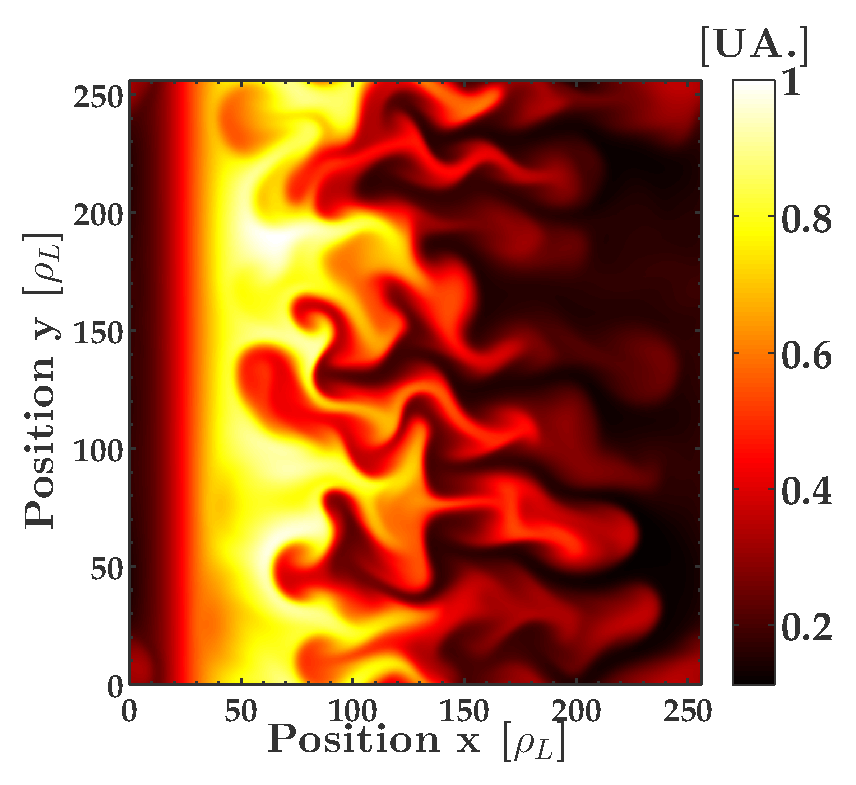
\includegraphics[height=6cm]{figures/2-CarteDensiteBase.eps}}
    \subfigure[]{\label{2-CartePotentielBase}
    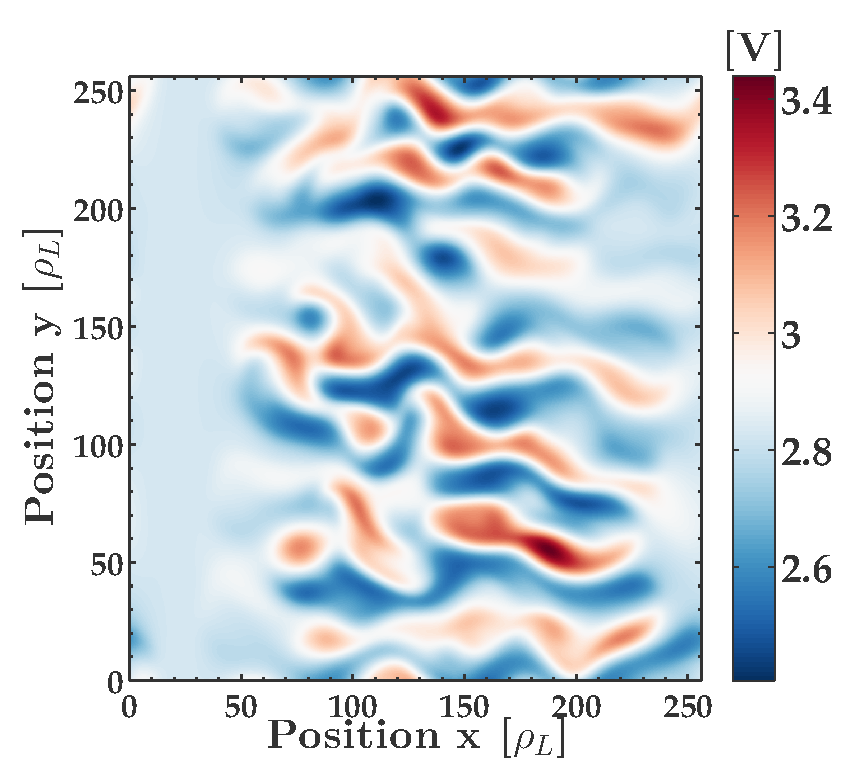
\includegraphics[height=6cm]{figures/2-CartePotentielBase.eps}}
    \caption{Cartes de la densité \subref{2-CarteDensiteBase}~~et du potentiel
    électrostatique
    \subref{2-CartePotentielBase}}
    \label{2-CartesBase}
\end{figure}

Quand l'équilibre est atteint, la nature de ce transport turbulent peut être
caractérisée statistiquement par des fonctions de distribution en probabilités
(PDF pour Probability Distribution Function) des différentes valeurs. 
 \begin{figure}[!htbp]
\centering
    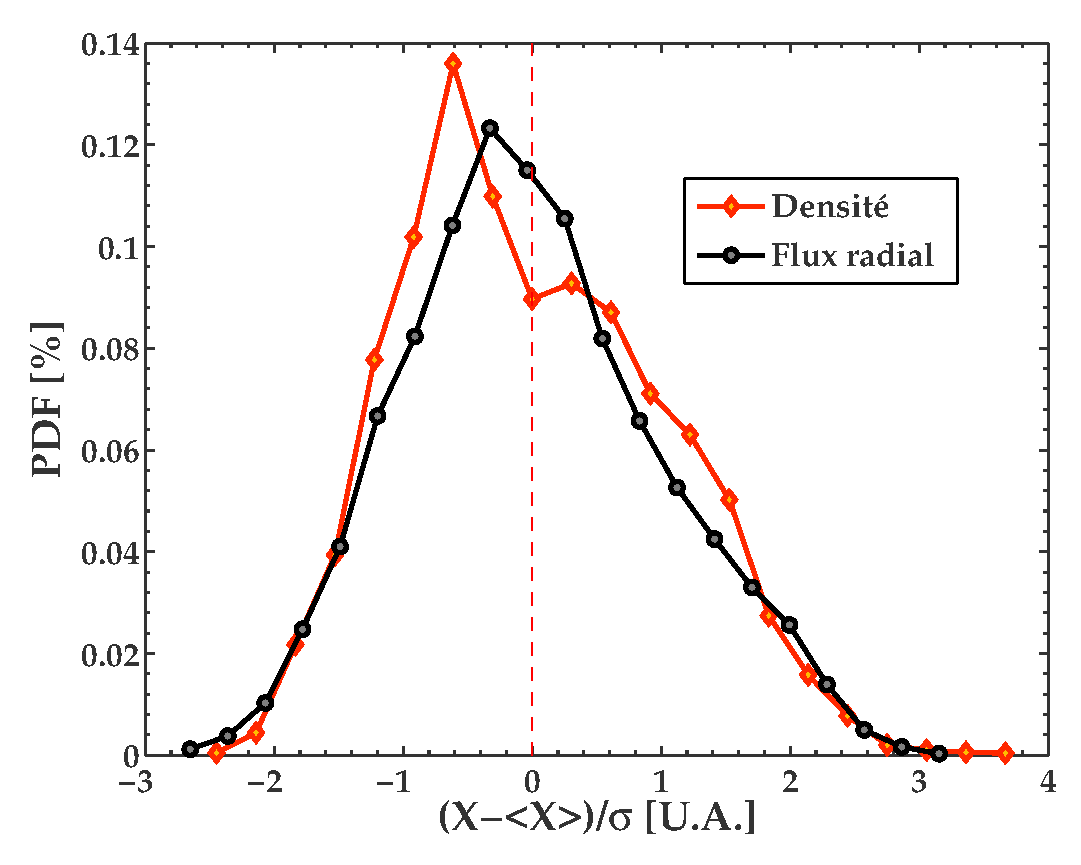
\includegraphics[width=8cm]{figures/2-PDFBase.eps}
    \caption{Densité de probabilité pour la densité et le flux radial}
    \label{2-PDFBase}
\end{figure}
 Les PDF
de la densité et du flux radial sont présentées sur la figure~\ref{2-PDFBase}. Elles
sont calculées proches de la source, à X$\sim$80$\rho_\text{L}$, sur un
échantillon statistique de 2000 pas de temps et moyennées suivant la direction
poloïdale. La PDF est centrée autour la valeur moyenne de la grandeur,
normalisée par son écart type, et donne en pourcentage la fréquence d'apparition
des fluctuations en fonction de leur importance.


Sur ces PDF on voit par exemple que la densité est le plus souvent
légèrement inférieure à la densité moyenne, et que des évènements plus
importants, de 3 à 4 fois l'écart type, peuvent apparaître. La PDF du flux
montre un phénomène caractéristique de l'instabilité d'interchange : bien que
les avanlanches donnent l'impression que le transport moyen soit dirigé dans
le sens des X croissants, le flux statistique le plus probable correspond aux
trous de plasmas qui remontent le gradient de densité.

Dans cette partie, nous avons présenté le modèle de base et le type
de solution que calculait TOKAM2D. Nous allons maintenant détailler les
modifications qui lui ont été apportées lors de la première année de ce travail
de thèse.

\section{Vers une description des sources d'ions}

Le modèle de TOKAM2D, dans la version que nous venons de présenter, n'est pas
directement applicable aux plasmas des sources d'ions. En effet dans
ces plasmas :

\begin{itemize}
	\item l'influence des parois sur le transport est primordiale. Des conditions
	aux limites périodiques, si elles sont acceptables dans le cadre de l'étude de
	l'instabilité d'interchange, ne peuvent pas représenter le champ électrique
	ambipolaire qui résulte de la chute de potentiel dans la gaine.
	\item le champ magnétique peut avoir une géométrie plus complexe et présenter
	de forts gradients.
	\item L'ionisation, processus contrôlant le bilan de particules, est fortement
	dépendante de la température électronique. Un modèle isotherme est donc
	intrinsèquement inadapté pour capturer la physique des sources d'ions.
\end{itemize}

Dans cette partie, nous présentons les évolutions successives du modèle pour
tenir compte de ces trois points.
Si les simulations de cette version complétée de TOKAM2D ne correspondent pas
encore aux plasmas froids des sources d'ions, elles seront tout de même
éclairantes sur le type de
transport qui se met en place dans des configurations de type filtre magnétique
et colonne de plasma pour des cas limites de notre étude, ie. où le plasma
est totalement ionisé et très magnétisé\footnote{La levée de ces deux hypothèses, qui n'est possible qu'en incluant l'interaction avec les atomes neutres, requiert une réécriture
plus en profondeur du modèle, ce qui sera l'objet de la partie suivante.}.

Dans le cadre de la recherche sur la fusion, cette refonte de TOKAM2D a tout
d'abord permis de vérifier les approximations choisies dans la description de
l'interchange du modèle original. Mais plus intéressant, les nouvelles
possibilités offertes par le code a ouvert la voie à de nouvelles études sur le transport du courant
et l'influence de la température électonique.

\subsection{Etude sur les conditions aux limites}
	
	Lors de l'étude du mouvement des fluides, le type d'écoulement qui se
	forme est toujours fortement dépendant de la géométrie du système et des conditions aux limites
	imposées par l'environnement. Cette considération est aussi vraie dans le
	cas des plasmas dont l'évolution est totalement contrôlée par l'interaction
	avec les parois. Celle-ci est décrite par la théorie classique des gaines,
	qui nous donne directement accès à la valeur des flux et des courants à la
	frontière du plasma, et nous fournit des conditions aux limites concrètes
	reflétant la réalité physique.
	
	En présence d'un champ magnétique, le courant se referme essentiellement
	à travers les parois parallèles et le critère de Bohm reste valide.
	Hélas, nous avons vu §~\ref{1-gaines} que dans la direction
	perpendiculaire la situation est plus ambiguë ; bien que la théorie
	classique ne tienne pas, le système doit tout de même être refermé, ce qui
	implique un choix arbitraire de conditions aux limites. Mais avec quel impact sur le
	système? Ce choix a-t-il une influence sur le transport transverse en soi?
	Quels sont les effets des conditions aux limites courament utilisées?
	
	La figure~\ref{2-profileDenNoLimit} compare les profils de densité pour des
	conditions aux limites périodiques, implémentées dans la version initiale de
	TOKAM2D, et des conditions aux limites absorbantes que nous définissons par
	trois critères :
	
	\begin{itemize}
	  \item les particules sont perdues dans la gaine et aucun flux ne peut
	  provenir des parois 
	  \begin{equation}
	  	\Gamma_\text{N}\cdot\mathbf n>0
	  \end{equation}
	  \item Le
	potentiel est fixé au potentiel flottant, interdisant aux
	courants de sortir dans la direction transverse
	\begin{equation}
	  	\Phi_\Omega=\Lambda
	  \end{equation}
	\item La vorticité est totalement amortie au contact de la gaine 
	\begin{equation}
	  	W_\Omega=0
	  \end{equation}
	\end{itemize}
	
\begin{figure}[htbp]
\centering
    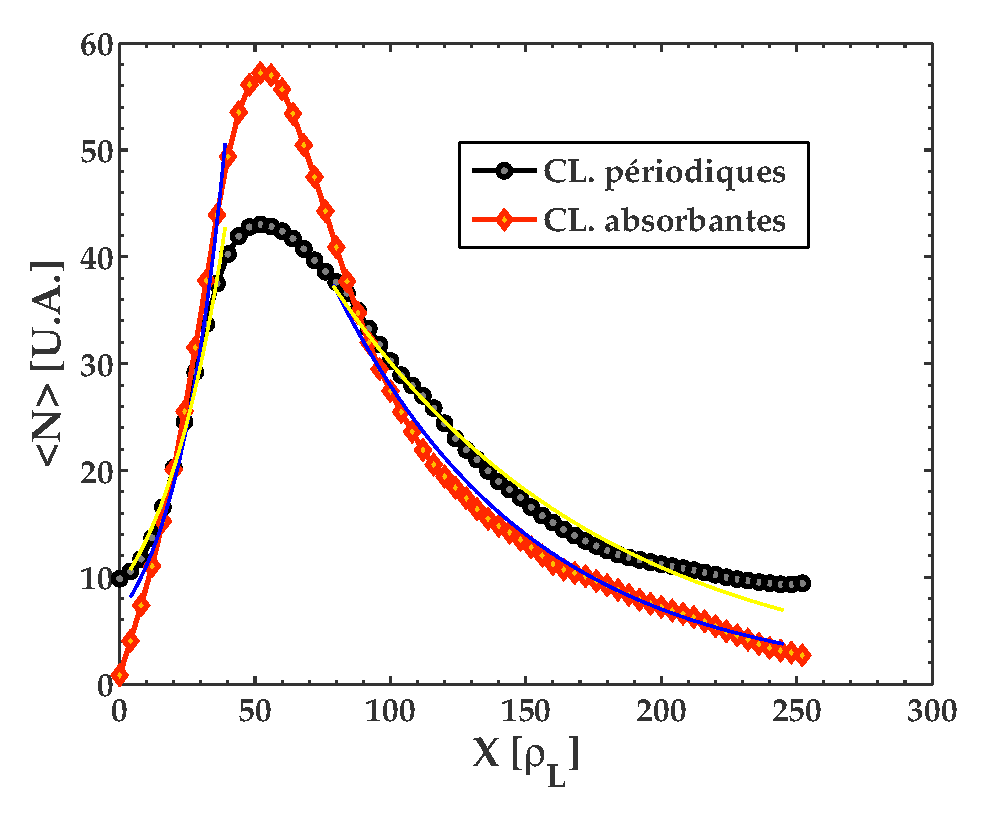
\includegraphics[width=8cm]{figures/2-profileDenNoLimit.eps}
    \caption{Profile de densité pour un cas périodique et un cas
    absorbant\label{2-profileDenNoLimit}}
\end{figure}
	Plusieurs différences sont à noter. Dans le cas périodique, la région stable
	est alimentée en particules par les flux traversant la fontière ; l'équilibre radial qui se
	forme est alors caractérisé par la combinaison des deux longueurs de
	décroissance.
	Dans le cas non-périodique, on peut voir que l'équilibre est indépendant de
	chaque côté de la source et que le profil de densité est aussi plus piqué. 
	
	Une analyse plus approfondie, publiée dans~\parencite{Futtersack-PSI} et
	jointe à ce manuscrit en annexe~\ref{AnnexeA}, étudie l'impact des conditions
	aux limites, parallèles et transverses, sur le courant et le transport en général.
	La conclusion prévient que la prise en compte de conditions aux limites
	physiques est obligatoire pour décrire correctement le transport qui s'installe
	dans les plasmas en général. Dans la direction parallèle, la conductivité de
	gaine joue un rôle crucial, prouvant la nécéssité d'opter pour des conditions
	aux limites issues de considération physiques. Dans la direction
	perpendiculaire, en attendant qu'une théorie solide se développe, il faut être
	conscient de l'influence du choix de ces conditions.
	
	TOKAM2D ayant été initialement
	développé avec une méthode spectrale, l'implémentation de conditions aux
	limites non-périodiques a nécéssité une réécriture presque complète du code.
	La nouvelle version est maintenant basée sur une méthode Volumes Finis, avec un
	schéma d'advection MUSCL (Modified Upwind Scheme for Conservation Laws),
	pouvant supporter les chocs, les discontinuités et les forts gradients. Les
	conditions aux limites ont été implémentées de façons très souples afin de
	pouvoir choisir entre différentes combinaisons :
	\begin{equation}
	\label{2-BC}
		\alpha \partial^2_{x}X + \beta \partial_{x}X + \gamma X =
		\delta
	\end{equation}
	$X$ pouvant représenter la densité, le potentiel ou la vorticité. A l'aide de
	l'expression~\ref{2-BC}, le quadruplet \{0,0,$\gamma$,$\delta$\} définit une
	condition aux limites de Dirichlet, et \{0,$\beta$,0,$\delta$\} une de
	Neumann, toutes combinaisons étant possibles.
	
	\subsection{Inclusion d'un champ magnétique non uniforme}
	
	Dans la version initiale
	des équations, l'effet de courbure du champ magnétique n'apparaît qu'à travers
	le coefficient de courbure $g$, tous les autres termes ayant été négligés.
	La deuxième évolution du modèle a consisté à inclure un champ magnétique
	inhomogène en espace pour élargir le domaine de fonctionnalité de TOKAM2D. Pour
	cela, nous reprenons les équations dérivées précédement, avant le développement
	des divergences. La version Volumes Finis de TOKAM2D utilisant un schéma
	d'advection évolué, les flux sont calculés de façon conservative et incluent
	directement l'effet de courbure du champ magnétique :
\begin{align}
\label{2-eqContinuiteMag}
&\partial_t \text{N}
= - \nabla\cdot\left(\text{N}\mathbf U_\text{E}\right) -\sigma
\text{N}e^{\Lambda-\Delta\Phi} + D\nabla^2 \text{N} + S
\\
\label{2-eqCourantMag}
&\partial_\text{t}\text{W} = 
-\nabla\cdot\left(\text{W}\mathbf U_\text{E}\right)
+\text{B}^2\sigma\left(1-e^{\Lambda-\Delta\Phi}\right) 
-\frac{\text{B}^2}{\text{N}}\nabla\cdot\left(\text{N}\mathbf U^i_*\right) 
+\nu\nabla_\perp^2\text{W}
\end{align}

Pour profiter de la nullité mathématique du rotationnel du gradient de
pression dans l'expression de la divergence du courant
diamagnétique, nous remarquons que celle-ci est équivalente à l'advection de la
densité par une vitesse fluide $\mathbf U_{\nabla\text{B}}$ :

\begin{equation}
\nabla\cdot\left(\text{N}\mathbf U_{\nabla\text{B}}\right)=
\nabla\cdot\left(\frac{2\text{N}\text{T}_e}{\text{B}^2}\nabla\text{B}\times\mathbf
b\right)
\end{equation}

Cette vitesse ressemble étonnement à la vitesse de dérive due au gradient du
champ magnétique que l'on rencontre dans la théorie particulaire du centre
guide. 

Pour illustrer la modification du code, nous simulons le cas d'une
barrière magnétique. Sur la
figure~\ref{2-CartesMagBarrier}, on observe le profil du champ magnétique : égal
à 0.1T et légèrement décroissant sur l'ensemble du domaine, la barrière est
placée en $\text{X}\sim$ 200$\rho_\text{L}$ et monte jusqu'à 0.2T à son maximum.

	\begin{figure}
    \centering
    \subfigure[]{\label{2-CarteDensiteMagBarrier}
    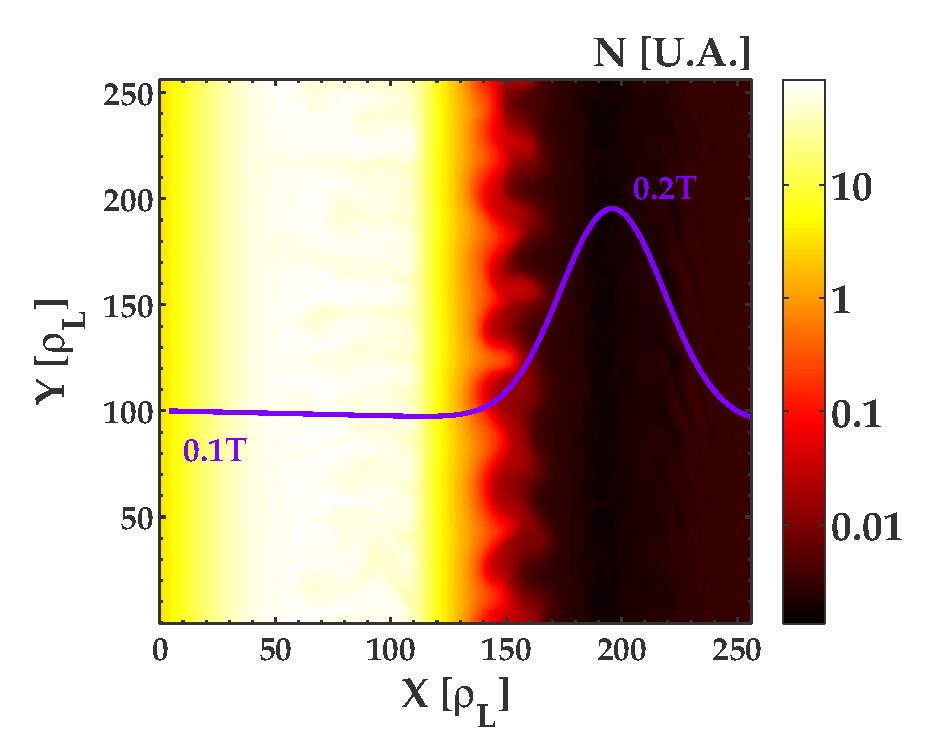
\includegraphics[height=5.8cm]{figures/2-CarteDensiteMagBarrier.eps}}
    \subfigure[]{\label{2-CartePotentielMagBarrier}
    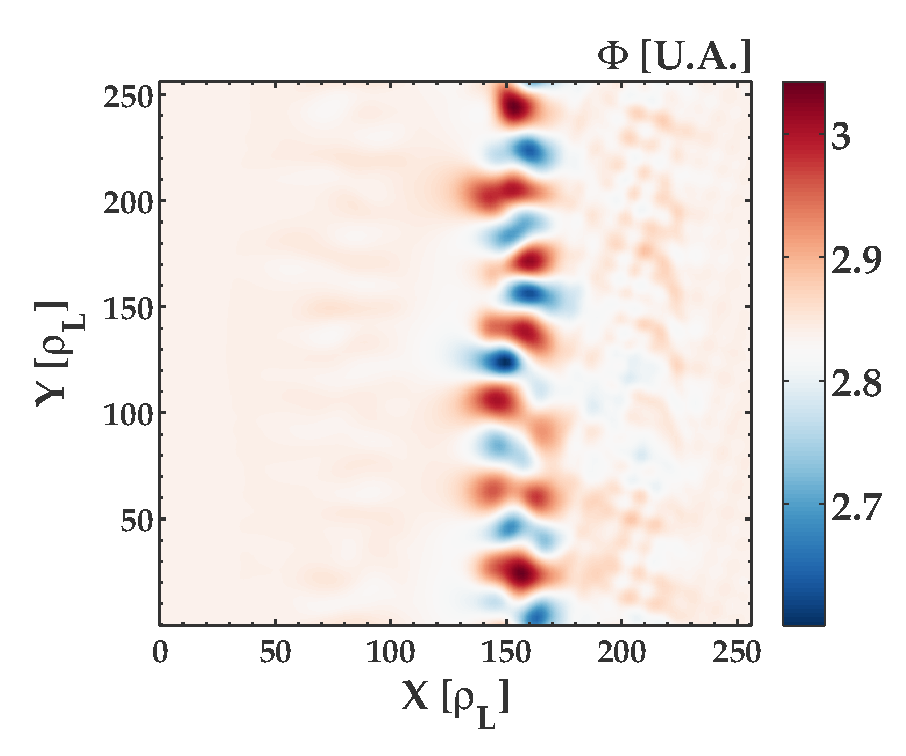
\includegraphics[height=5.8cm]{figures/2-CartePotentielMagBarrier.eps}}
    \caption{Cartes de densité \subref{2-CarteDensiteMagBarrier} et de potentiel
    \subref{2-CartePotentielMagBarrier}}
    \label{2-CartesMagBarrier}
\end{figure}

On voit que la barrière est très efficace. La carte de densité, prise en log,
montre des vaguelettes qui se déplacent rapidement dans la direction poloïdale.
Au même endroit, le potentiel forme lui aussi des structures qui s'étalent le
long du gradient positif de champ magnétique. 
Dans cette simulation, c'est le cisaillement de cette vitesse de dérive qui
apparaît dans la direction poloïdale qui semble responsable de l'effet de
barrière. 


	\subsection{Implémentation de l'équation d'énergie}
	La fermeture isoterme choisie dans le modèle de TOKAM2D est aussi très
	discutable. Comme le potentiel plasma est fortement lié à la température
	électronique à travers les conditions de gaines, il a tendance à suivre ses
	fluctuations. Le transport transverse dans la SOL peut alors se voir grandement
	impacté par l'apparition d'un gradient radial de température qui donne alors
	naturellement naissance à une dérive poloïdale. De plus, la prise en compte des
	variations spatiales de la température complexifie énormément la relation de
	dispersion obtenue par analyse linéaire du modèle, et peut donner lieu à
	l'apparition d'instabilités différentes de l'interchange.
	
	Pour obtenir l'équation de la température électronique, nous partons de
	l'équation de conservation de l'énergie normalisée :
	
	\begin{equation} 
		\frac{3}{2}\partial_t \text{P}_e +
		\frac{3}{2}\nabla\cdot\left(\text{P}_e\mathbf{U}+\mathbf{Q}\right) +
		\text{P}_e\nabla\cdot\mathbf{U}=S_{\text{T}_e} +
		\mathbf{\Pi}:\nabla \mathbf U
	\end{equation}
	
	Les équations du modèle s'écrivent alors :
	
\hspace*{-2cm}\begin{minipage}{1.1\textwidth}
\begin{align}
\label{2-eqContinuiteTemp}
&\partial_t \text{N}
= - \nabla\cdot\left(\text{N}\mathbf U_\text{E}\right) -\sigma
\text{N}\sqrt{\text{T}_e}e^{\Lambda-\Delta\Phi/\text{T}_e} + D\nabla^2 \text{N}
+ S
\\
\label{2-eqCourantTemp}
&\partial_\text{t}\text{W} = 
-\nabla\cdot\left(\text{W}\mathbf U_\text{E}\right)
+\text{B}^2\sigma\sqrt{\text{T}_e}\left(1-e^{\Lambda-\Delta\Phi/\text{T}_e}\right)
-\frac{\text{B}^2}{\text{N}}\nabla\cdot\left(\text{N}\mathbf
U_{\nabla\text{B}}\right) +\nu\nabla^2\text{W}
\\
\label{2-eqEnergyTemp}
&\partial_\text{t}\text{P}_e 
+\nabla\cdot\left(\text{P}_e\mathbf U_\text{E}\right) =
\text{NT}_e\sigma\sqrt{\text{T}_e}e^{\Lambda-\Delta\Phi/\text{T}_e}
-\frac{2}{3}\text{P}_e\nabla\cdot\mathbf U
+\chi\nabla^2\text{P}_e
+\frac{2}{3}S_{\text{T}_e}
\end{align}
\end{minipage}

	\begin{figure}
    \centering
    \subfigure[]{\label{2-CarteDensiteWithTe}
    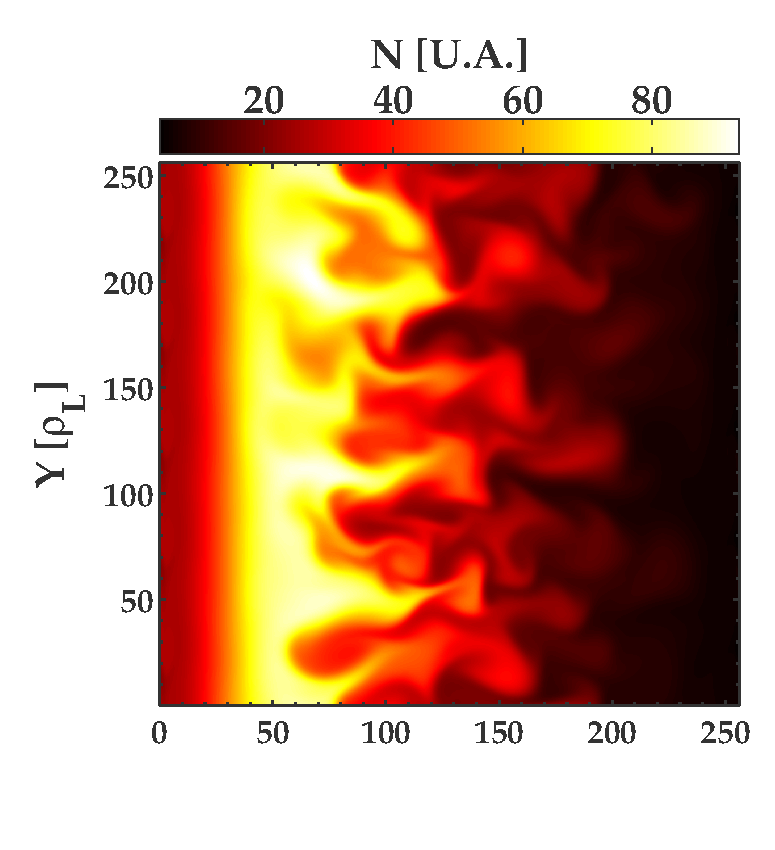
\includegraphics[height=5.75cm]{figures/2-CarteDensiteWhTe.eps}}
    \subfigure[]{\label{2-CartePotentielWithTe}
    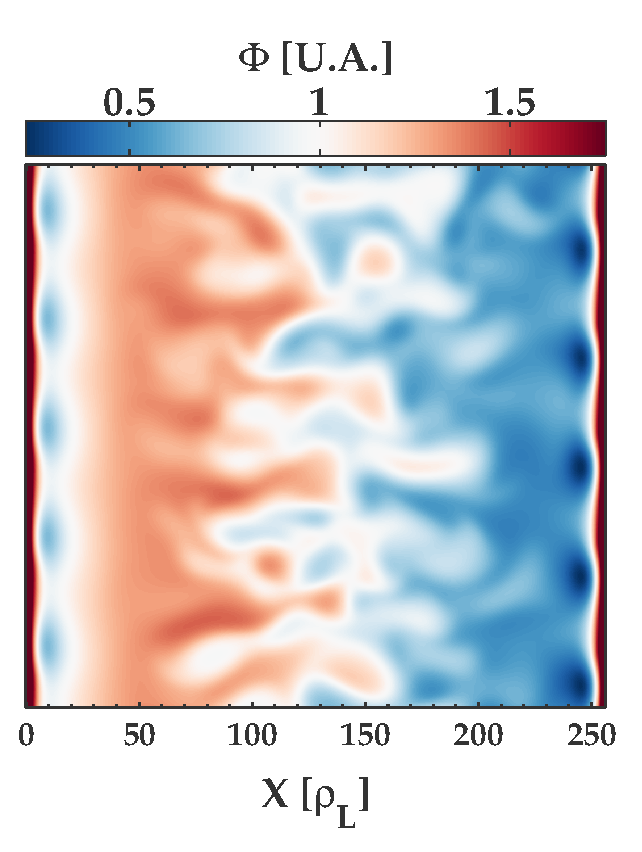
\includegraphics[height=5.75cm]{figures/2-CartePotentielWhTe.eps}}
    \subfigure[]{\label{2-CarteTeWhTe}
    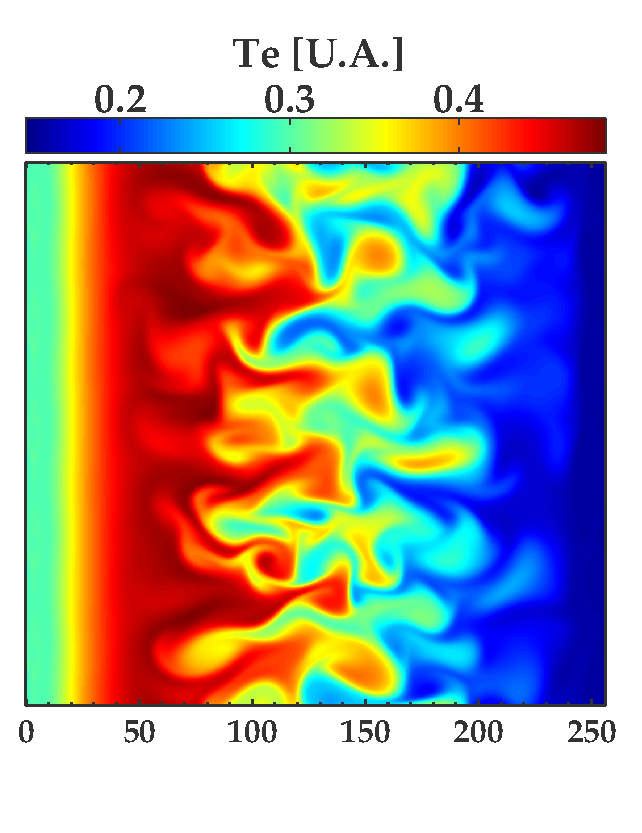
\includegraphics[height=5.75cm]{figures/2-CarteTeWhTe.eps}}
    \caption{Cartes de densité \subref{2-CarteDensiteBase}, de potentiel
    \subref{2-CartePotentielBase} et de température \subref{2-CarteDensiteBase}}
    \label{2-CartesWithTe}
	\end{figure}
	
	\begin{figure}[htbp]
\centering
    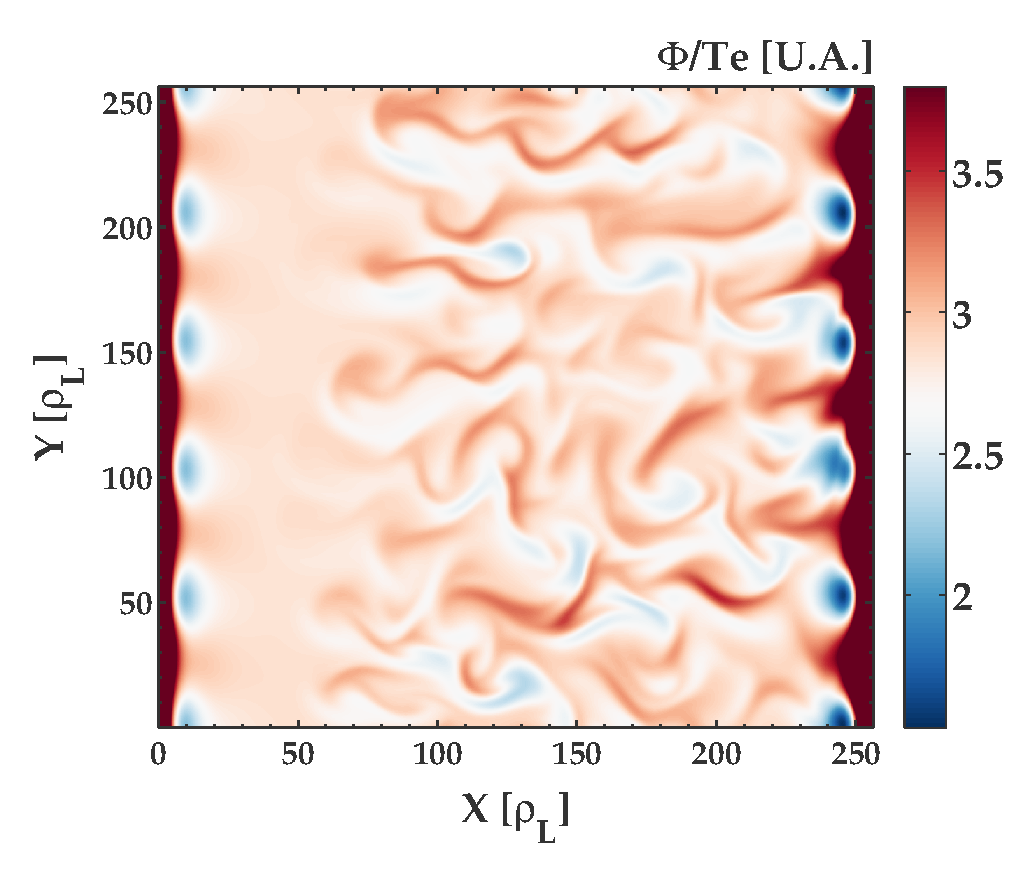
\includegraphics[width=10cm]{figures/2-CartePotentielSurTeWhTedNdx.eps}
    \caption{Carte du potentiel électrostatique rapporté à la température.}
    \label{2-CartePotentielSurTeWhTedNdx}
\end{figure}

	
	\subsubsection{Impact sur le transport transverse}
	
	\begin{figure}[htbp]
    \centering
    \subfigure[]{\label{2-CarteDensiteWhTe}
    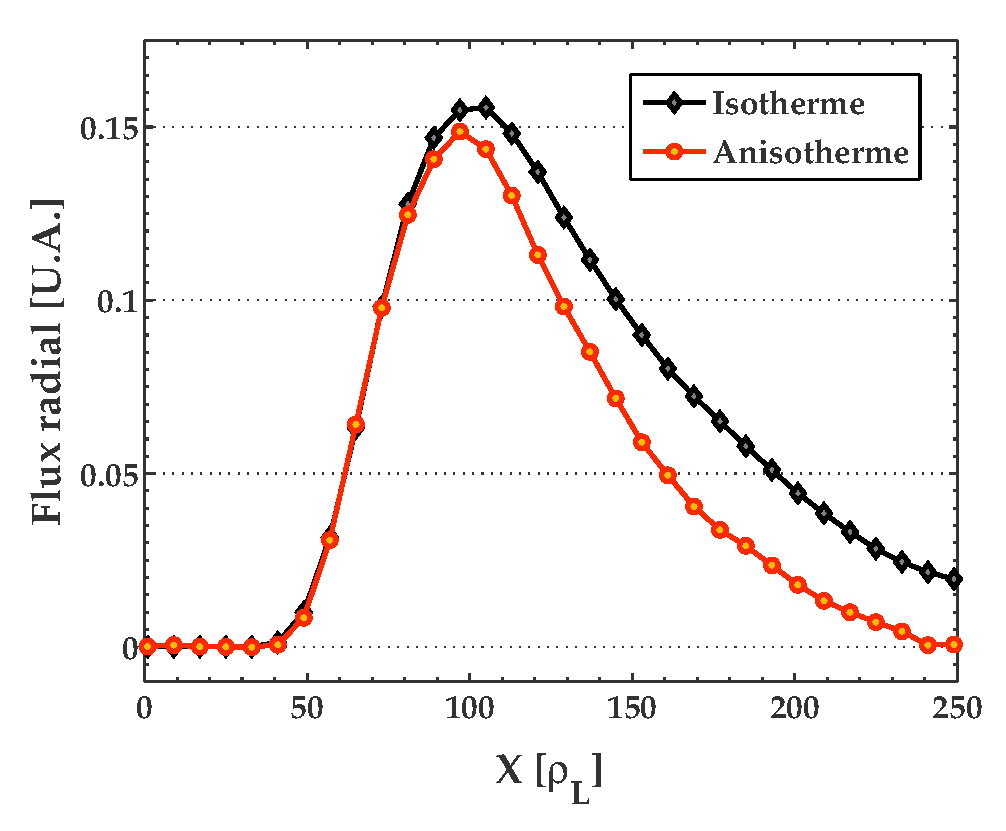
\includegraphics[height=5cm]{figures/2-profileFluxRadialWhTedNdx.eps}}
    \subfigure[]{\label{2-profileFluxRadialWhTedNdx}
    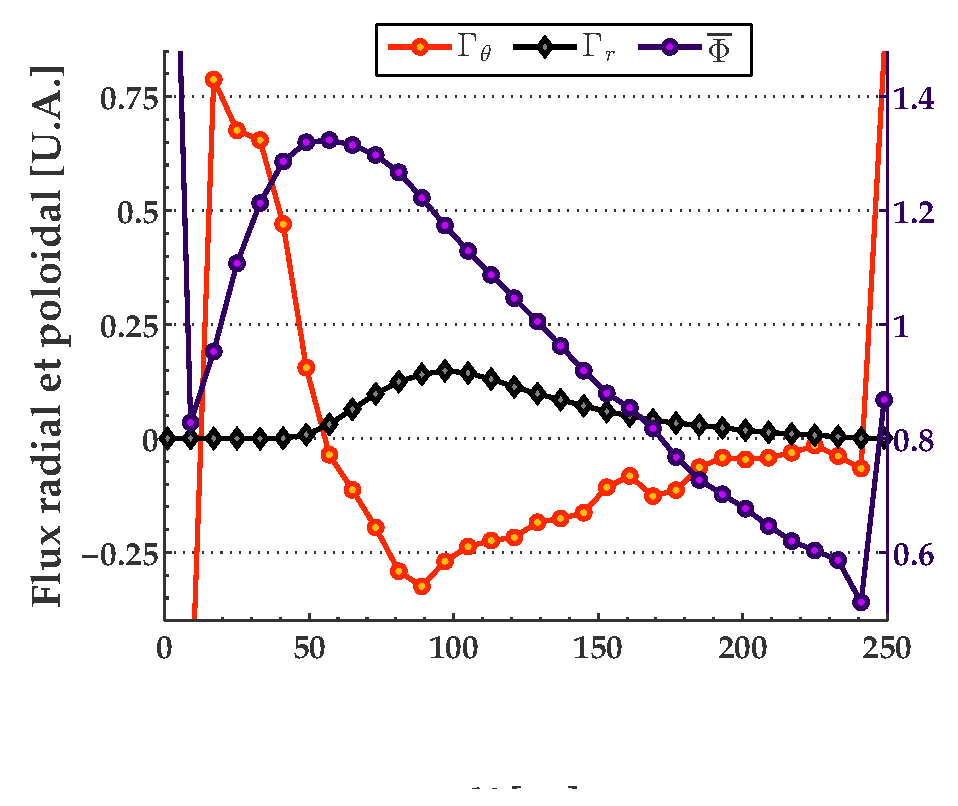
\includegraphics[height=6cm]{figures/2-profileFluxWhTedNdx.eps}}
    \caption{Cartes de densité \subref{2-CarteDensiteWhTe}, de potentiel
    \subref{2-CartePotentielBase} et de température \subref{2-profileFluxWhTedNdx}}
    \label{2-CartesWithTe}
	\end{figure}
	
	\subsubsection{Application au filtre magnétique}
	\begin{figure}[htbp]
    \centering
    \subfigure[]{\label{2-CarteDensiteMagBarrierWhTe}
    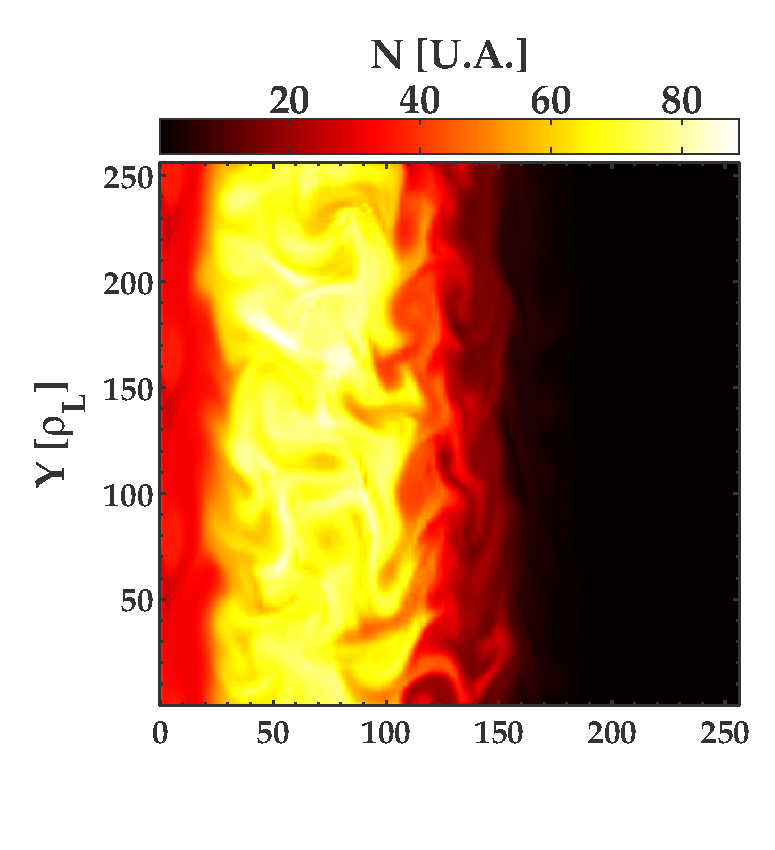
\includegraphics[height=5.75cm]{figures/2-CarteDensiteMagBarrierWhTe.eps}}
    \subfigure[]{\label{2-CartePotentielMagBarrierWhTe}
    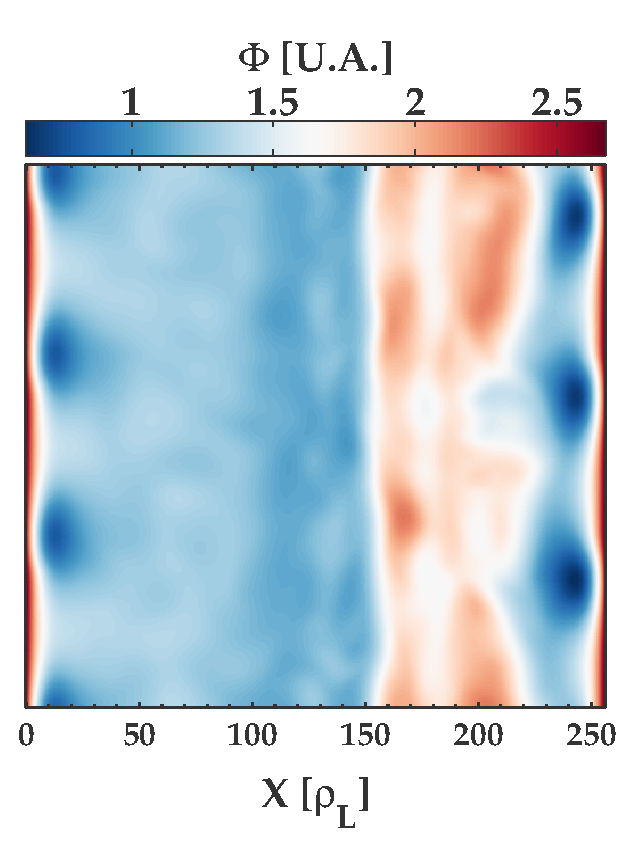
\includegraphics[height=5.75cm]{figures/2-CartePotentielMagBarrierWhTe.eps}}
    \subfigure[]{\label{2-CarteTeMagBarrierWhTe}
    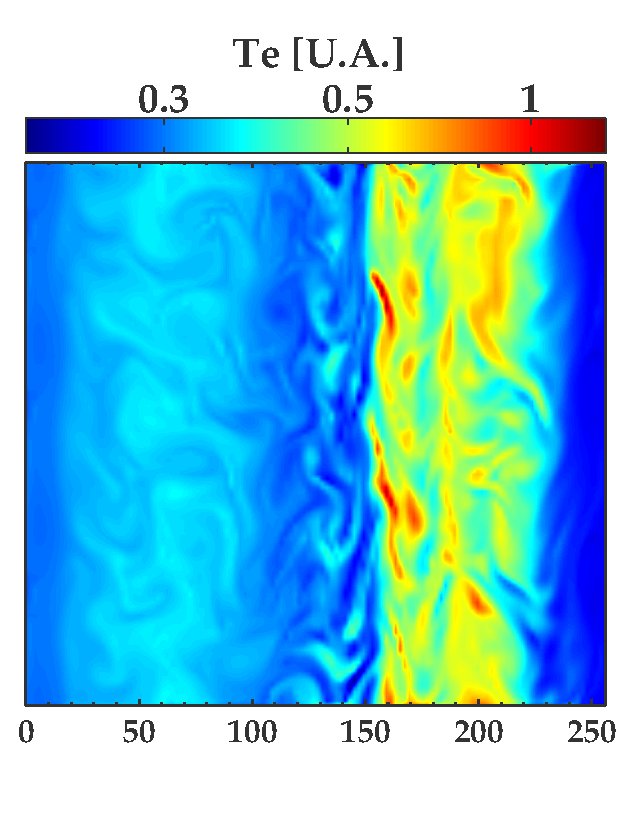
\includegraphics[height=5.75cm]{figures/2-CarteTeMagBarrierWhTe.eps}}
    \caption{Cartes de densité \subref{2-CarteDensiteMagBarrierWhTe}, de potentiel
    \subref{2-CartePotentielMagBarrierWhTe} et de température \subref{2-CarteTeMagBarrierWhTe}}
    \label{2-CartesWithTe}
	\end{figure}
	
	\subsubsection{Simulation d'une colonne de plasma magnétisée}
	
	\begin{figure}[htbp]
    \centering
    \subfigure[]{\label{2-CarteDensiteMagColumn}
    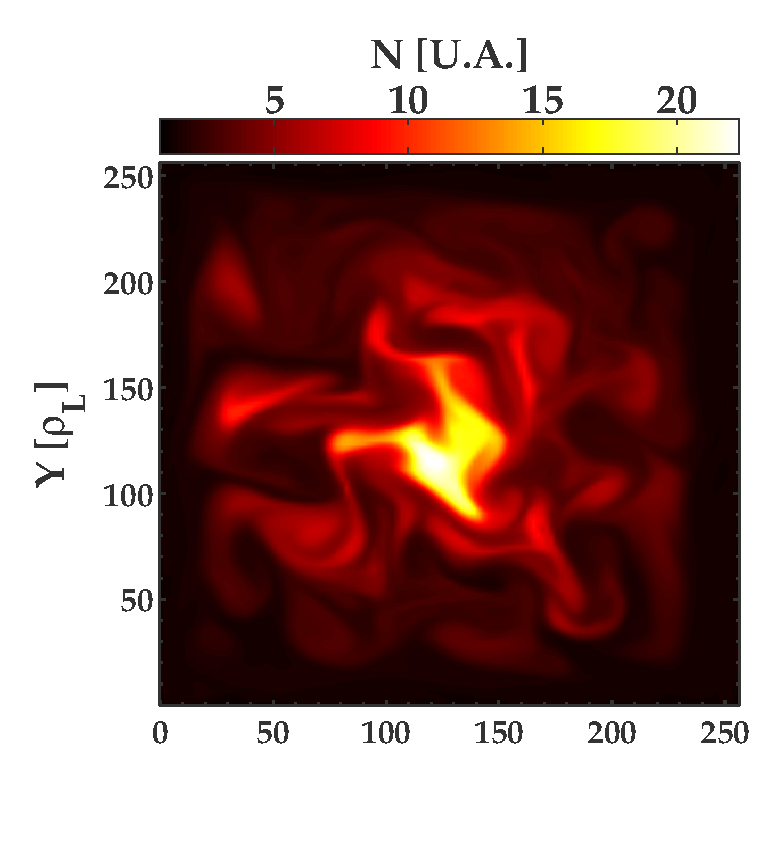
\includegraphics[height=5.75cm]{figures/2-CarteDensiteMagColumn.eps}}
    \subfigure[]{\label{2-CartePotentielMagColumn}
    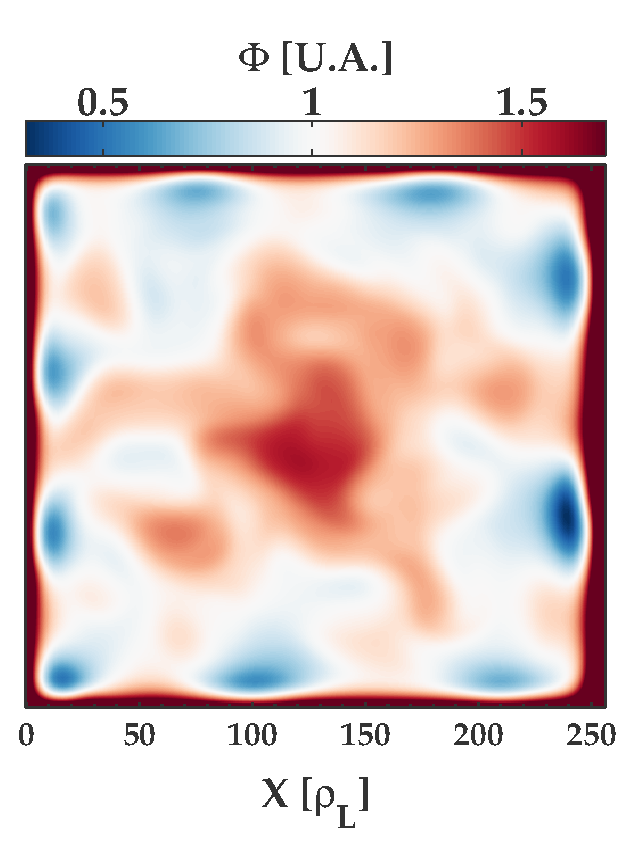
\includegraphics[height=5.75cm]{figures/2-CartePotentielMagColumn.eps}}
    \subfigure[]{\label{2-CarteTeMagColumn}
    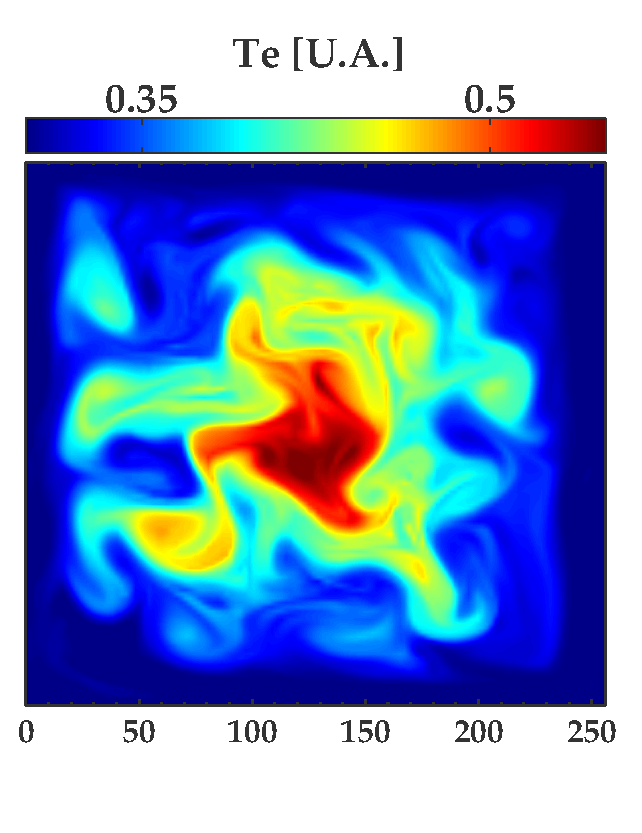
\includegraphics[height=5.75cm]{figures/2-CarteTeMagColumn.eps}}
    \caption{Cartes de densité \subref{2-CarteDensiteMagColumn}, de potentiel
    \subref{2-CartePotentielMagColumn} et de température \subref{2-CarteTeMagColumn}}
    \label{2-CartesWithTe}
	\end{figure}
\section{L'approche par vitesses de dérive pour les plasmas
froids}
\label{vitessesDerivePlasmaFroid}
Les équations de TOKAM2D ne décrivent pas non plus l'intéraction
collisionnelle des particules chargées avec la population neutre, essentielle dans la physique des plasmas froids,
\begin{figure}[htbp]
    \centering
    \subfigure[]{\label{2-CarteDensiteMapl}
    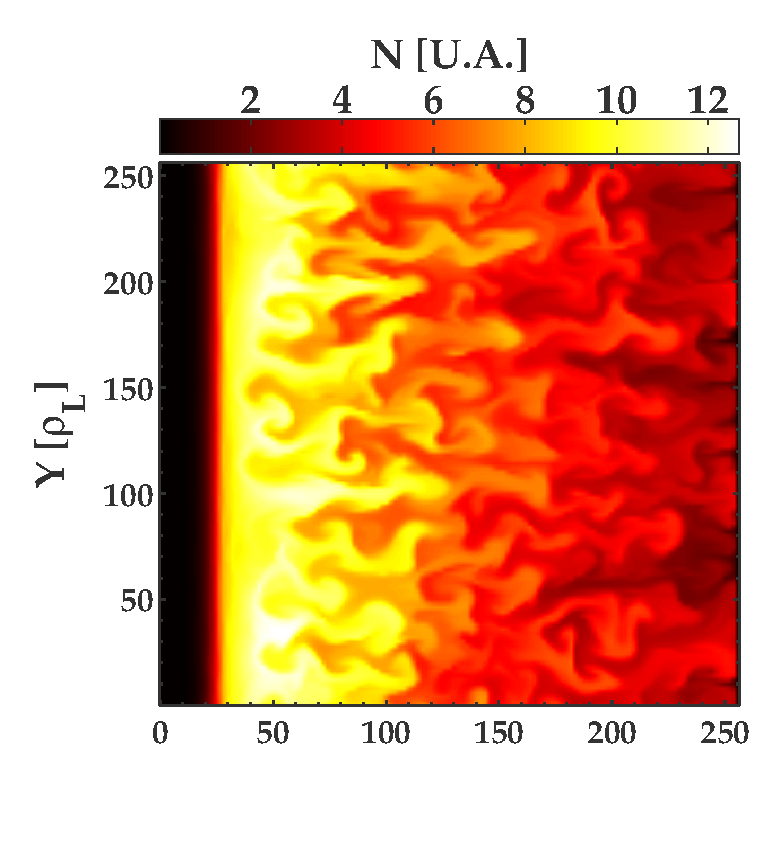
\includegraphics[height=8cm]{figures/2-CarteDensiteMapl.eps}}
    \subfigure[]{\label{2-CartePotentielMapl}
    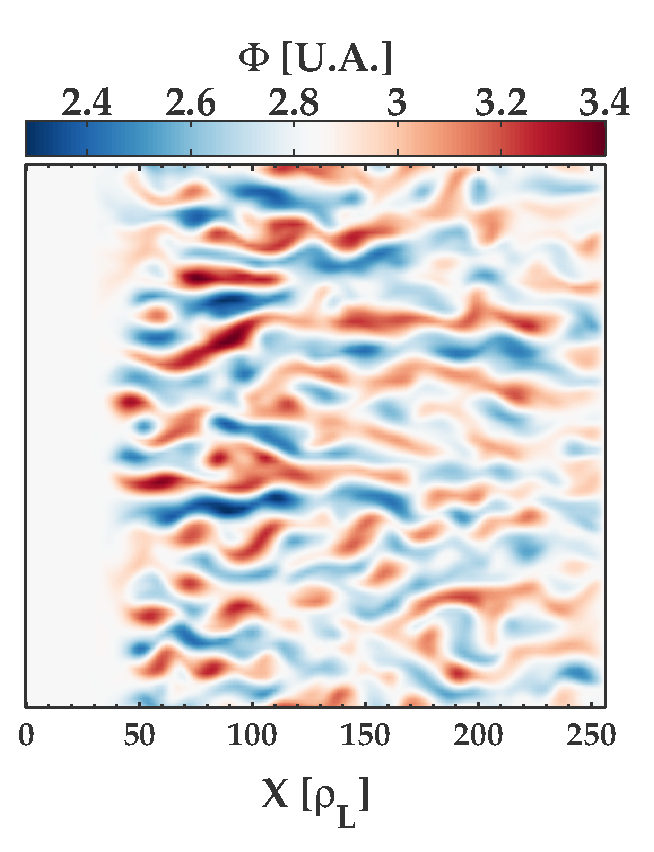
\includegraphics[height=8cm]{figures/2-CartePotentielMapl.eps}}
    \caption{Cartes de densité \subref{2-CarteDensiteMapl}~~et de potentiel
    \subref{2-CartePotentielMapl}}
    \label{2-CartesWithTe}
	\end{figure}
%\bibliographystyle{apalike}
%\bibliography{biblio}

\end{refsection}




